\subsubsection{Housing Cooperatives}
\label{sec:brf}

\paragraph{Aim and target group}

The housing cooperative part of the application is used by housing cooperatives in \textit{Hammarby Sj{\"o}stad}, Stockholm Test Site. This part provides features for building level energy information and actions. 

 All apartment owners in Sweden have to be members of a housing cooperative that owns the building. A board is elected among the members and the board is in charge of the cooperative's finances and maintenance of the building. This work may include deciding on energy contracts, making sure energy systems are maintained and proposing investments in more energy efficient technologies. People in the board are volunteers who may have no previous knowledge of energy or building management. Hence, the housing cooperative part of the app aims to support board members in energy management work and, more specifically, in taking energy reduction actions.

In Hammarby Sj{\"o}stad, some of the housing cooperatives have an appointed energy manager in the board who is responsible for the energy work. This role, no matter if it is explicitly named energy manager or if it is an implicitly shared responsibility among several board members, is the primary target for the housing cooperative part of the app. The app can also be used by other housing cooperative members who are interested in following the energy work of the cooperative. A third type of user is energy or building management companies working with housing cooperatives. All information in the app is visible for all these user groups and shared between housing cooperatives. This openness of energy data is key to facilitating the users in sharing experiences relevant for taking energy reduction actions.

\paragraph{Linking energy data to energy reduction actions}

One of the main housing cooperative features of the app is that it allows for linking energy data with energy reduction actions taken, which makes it possible to follow up on the impact of energy actions (see Figure \ref{fig:Figure201_Actions}). The energy use is divided into heating and hot water (from district heating) and facilities electricity and the user can switch between these views in the energy use graph (see Figure \ref{fig:Figure201_Actions}, left). The user can also choose between viewing energy use per month or per year. This provides enough level of detail to show overall changes in energy use. Since the energy data is shared between cooperatives there may also be privacy concerns related to opening up data of higher granularity to people outside of the own cooperative. 

\begin{figure}
	\centering
	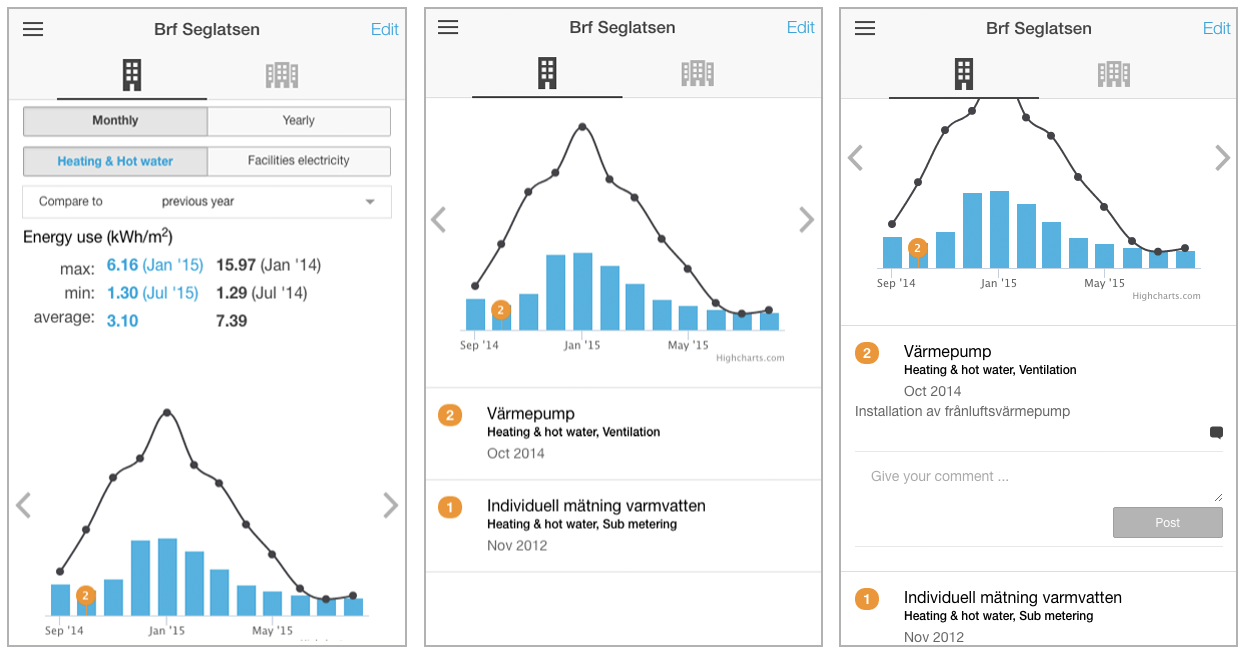
\includegraphics[width=0.98\linewidth]{img/Figure201_Actions.png}
	\caption{Energy use graph where the blue bars show the current year's energy use and the black line shows the previous year's energy use. Energy reduction actions taken are mapped to the graph and listed below.}
	\label{fig:Figure201_Actions}
\end{figure}

Users with editing rights, typically energy managers or other boards members, can in the app add energy reduction actions that the cooperative has taken, including information about:
\begin{itemize}
\item Title of the action.
\item Type of energy action (e.g. heating optimisation, action affecting the ventilation or action to make lighting more efficient). The action types are in the form of tags (more than one can be added to each action), which makes it possible to add functionality for filtering or searching for specific actions.
\item Month and year the action was taken or completed.
\item Cost for taking the action.
\item Additional details about the action.
\end{itemize}

Energy or building management companies that work with a cooperative can also get editing rights and add energy reduction actions they take on behalf of the cooperative. Added actions appear in the energy use graph at the month when each action was taken and all actions are listed below the graph. When clicking on an action in the list, the action is expanded and the details of the action are shown.

To make the impact of energy reduction actions visible, the user can choose to compare the energy use of the viewed months to the energy use of the same months the previous year. This can be used for example when a housing cooperative wants to explore what energy reduction actions to take in the future by looking at the actions taken by other cooperatives and what the effects were in relation to costs.

\paragraph{Comparing housing cooperatives}

\begin{figure}
	\centering
	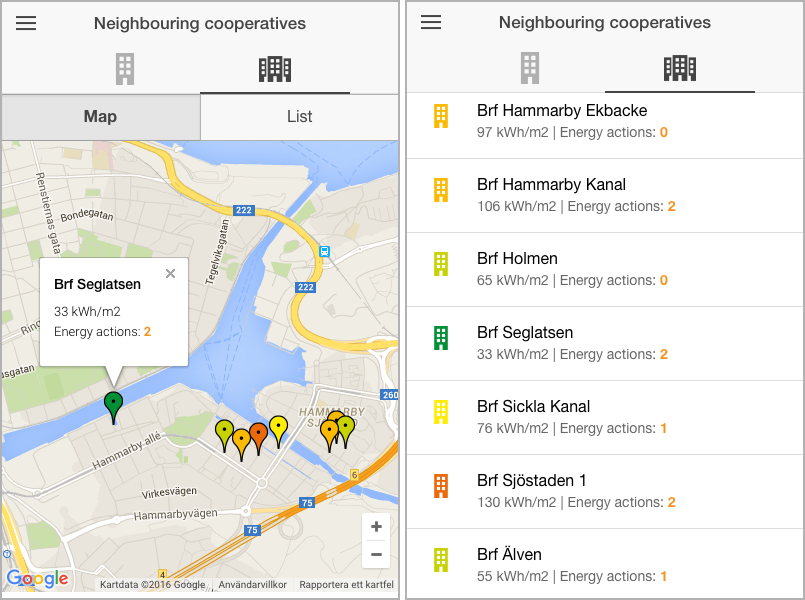
\includegraphics[width=0.9\linewidth]{img/Figure202_Housing_cooperatives_comparison.png}
	\caption{Map and list view of participating housing cooperatives. The energy performance of the cooperatives is indicated by colour and in numbers.}
	\label{fig:Figure202_Housing_cooperatives_comparison}
\end{figure}

A user can see all cooperatives who are using the app in a map view or list view (see Figure~\ref{fig:Figure202_Housing_cooperatives_comparison}). To facilitate comparison between cooperatives the icons in the map and list are colour coded based on each cooperative's energy performance, i.e. the energy use per square meter heated area (kWh/m$^2$). It uses a scale from red to green, where a red colour indicates a poor energy performance (i.e. high energy use) and a green colour indicates good energy performance (i.e. low energy use). The energy performance scale is calculated in a similar way as for the Swedish energy declaration for buildings\footnote{\url{http://www.boverket.se/sv/byggande/energideklaration/energideklarationens-innehall-och-sammanfattning/sammanfattningen-med-energiklasser/energiklasser-fran-ag/}}  but it is calibrated to only include measured energy use for heating and hot water, which is the greatest part of the energy use. In the Swedish energy declarations, facilities electricity is also added but that often requires estimations of different factors to make the number comparable.




For each cooperative in the list or on the map, the user can also see the energy performance as a number (kWh/m$^2$) and the number of energy reduction actions taken. The number of actions is important to display to make energy reduction efforts of housing cooperatives with a high energy performance (e.g. due to poor construction of the building) visible. 

The energy managers in the project stressed that it is important to know what type of housing cooperative you are comparing your own to, in order to understand what any differences in energy performance may depend on and which of their experiences could be relevant for the own cooperative. Therefore, the app provides the following information about each cooperative (see Figure \ref{fig:Figure203_cooperative_info}):
\begin{itemize}
\item Number of apartments in the cooperative.
\item The cooperative's heated area ($m^2$).
\item The building's construction year.
\item Type of ventilation (e.g. with or without heat recovery).
\end{itemize}

\begin{figure}
	\centering
	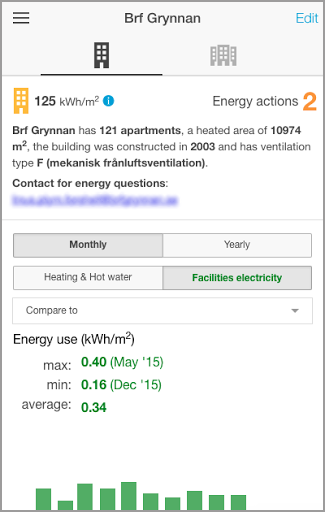
\includegraphics[width=0.4\linewidth]{img/Figure203_cooperative_info.png}
	\caption{Information about the housing cooperative that is important for understanding the energy performance and actions taken is displayed in the top of the page.}
	\label{fig:Figure203_cooperative_info}
\end{figure}

While the energy performance provides a comparison of the current situation, there is also a feature for comparing a cooperative's energy use over time to the neighbourhood average (see Figure \ref{fig:Figure204_Neighbourhood_average}). In the energy use graph for each cooperative, divided into heating and hot water and facilities electricity, the user can display the average energy use of the other cooperatives using the app. In that way, the user can get an idea of how a cooperative's energy use has changed over time in relation to other cooperatives. To make the energy use comparable between cooperatives, the energy in the graphs is (in the same ways as the energy performance) displayed as energy use divided by heated area (kWh/m$^2$).

\begin{figure}
	\centering
	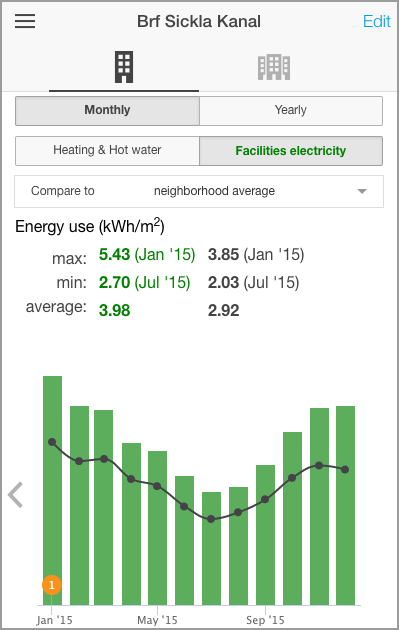
\includegraphics[width=0.4\linewidth]{img/Figure204_Neighbourhood_average.png}
	\caption{The green bars show the monthly facilities electricity use of the housing cooperative and the black line shows the average facilities electricity use for all housing cooperatives using the app.}
	\label{fig:Figure204_Neighbourhood_average}
\end{figure}

\paragraph{Sharing experiences}

The details about each energy action taken by a cooperative, together with the effects on the energy use, provides information that could support other cooperatives in learning more about which energy reduction actions are effective. However, a cooperative that is interested in taking an action may want more information than what is provided by the person adding the action, e.g. regarding how to take an action, which contractor was used for an investment or how to get buy-in from the cooperative members. The app supports this through a commenting function for each action added, where users can post questions related to the action. The cooperatives can also choose to add an email address to their energy contact person, which is visible on the cooperatives app page, to allow for direct contact.

Sharing of experiences of course also happens outside of the digital world, e.g. during housing cooperative board meetings or meetings with the local energy network in Hammarby Sj{\"o}stad. The app is aiming to support discussions and knowledge exchange also in such situations, and it should be easy for someone who wants to demonstrate the impact of an energy investment to just take out the smart phone and show the visualization. Consequently, the mobile screen format is an important part of the design.
